\documentclass{article}
    % General document formatting
    \usepackage[margin=0.7in]{geometry}
    \usepackage[parfill]{parskip}
    \usepackage[utf8]{inputenc}
    
    % Related to math
    \usepackage{amsmath,amssymb,amsfonts,amsthm}
\usepackage{graphicx}
%\usepackage{subfig}
%\usepackage{subfigure}
\usepackage{caption}
\usepackage{subcaption}
\usepackage{listings}

\usepackage{titling}
%\usepackage{lipsum}

\usepackage{titlesec}

\titleformat*{\section}{\large\bfseries}
\titleformat*{\subsection}{\large\bfseries}
%\titleformat*{\subsubsection}{\large\bfseries}
%\titleformat*{\paragraph}{\large\bfseries}
%\titleformat*{\subparagraph}{\large\bfseries}
\titlespacing\section{0pt}{6pt plus 3pt minus 2pt}{0pt plus 2pt minus 2pt}
\titlespacing\subsection{0pt}{6pt plus 3pt minus 2pt}{0pt plus 2pt minus 2pt}
\titlespacing\subsubsection{0pt}{6pt plus 3pt minus 2pt}{0pt plus 2pt minus 2pt}

\pretitle{\begin{center}\large\bfseries}
\posttitle{\par\end{center}\vskip 0.01em}
\preauthor{\begin{center}\Large\ttfamily}
\postauthor{\end{center}}
\predate{\par\normalsize\centering}
\postdate{\par}

%\title{GI Assignment 3: A study of \textit{RB1} variation and regulation}
%\date{\today}

\begin{document}

%\maketitle

\begin{center}
\textbf{\Large{\centering{Scientific Programming Assignment 3: Simulating spatial point patterns}}}\\
\vspace{0.8mm}
\textbf{\textit{\small{USN: 303039534}}}
\end{center}
\vspace{1.3mm}

\section{dmin2d}

We start by implementing the dmin2d model as described in the assignment and plot two examples of a dmin2d simulation with parameters n=200, m=30, s=5 and ranges of x=[200:1000] and y = [100:900] (figure 1).

\begin{figure}[h]
	\centering
	\begin{subfigure}[t]{0.33\linewidth}
		\centering
		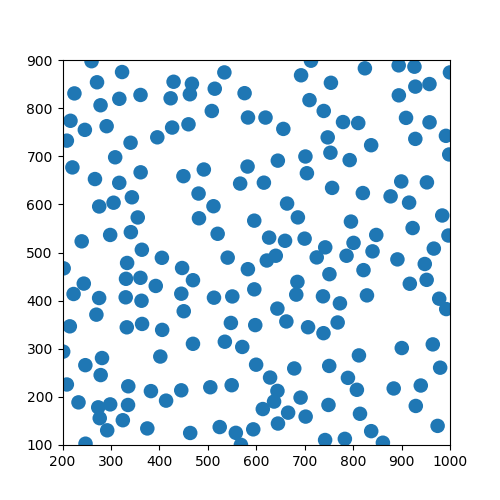
\includegraphics[width = 1.0\linewidth, trim={20 20 20 20}, clip=true]{dmin1.png}
		\subcaption{}
		\label{fig:dmin1}	
	\end{subfigure}
	\hspace{0.12\linewidth}
	\begin{subfigure}[t]{0.33\linewidth}
		\centering
		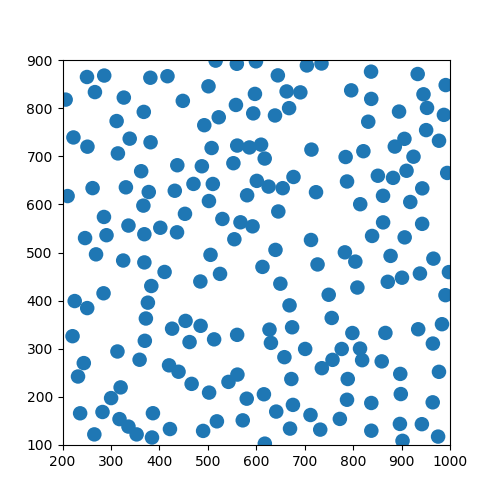
\includegraphics[width = 1.0\linewidth, trim={20 20 20 20}, clip=true]{dmin2.png}
		\subcaption{}
		\label{fig:dmin2}	
	\end{subfigure}
\label{fig:dmin}
\caption{Two examples of running the dmin2d model with n=200, m=30, s=5. The diameter used for plotting is the mean of the dmin model; pairs of points exhibiting overlap must thus have at least one point added with a dmin smaller than the mean.}
\end{figure}

\section{Regularity Index}

We proceed to implement a function \textit{calc\_RI()} to calculate the regularity index of a given pattern. The regularity index is defined as
\begin{equation}
	RI = \dfrac{\text{mean}(dmin(i))}{\text{stdev}(dmin(i))}
\end{equation} 
where $dmin(i)$ is the distance between point i and its nearest neighbor.
RI is a measure of how regular the local spacing of points is; if all points have similar nearest neighbor spacings, the standard deviation will be low and the regularity index high. If, on the other hand, pairwise distances differ a lot, the standard deviation will be high and the regularity index low. This is weighted by the mean nearest-neighbor distance to account for scalings of the grid.

For a given set of parameters, we can proceed to generate 1000 random patterns and calculate the regularity index of each pattern. We report the 50th largest value as a measure of regularity for this set of parameters.
This is the boundary between the 5\% highest and 95\% lowest regularity indices we generate given these parameters, and thus tells us how regular a pattern we can expect to generate within a reasonable number of trials (here 20) with these parameters.
In the following, we denote this regularity measure RI50 and calculate it with the function \textit{run\_sims()}.

We use \textit{run\_sims()} to calculate RI50 for a grid with n=200, m=0, s=0, x=[0:1000] and y=[0:1000]; that is for a square pattern of 200 points with no exclusion zone.
For this set of parameters, we find that RI50 = 2.070. Repeating the calculation 10 times we find a mean of 2.0695 with a standard deviation of 0.006 across trials.
This shows another benefit of the RI50 measure in that it is relatively consistent across trials in contrast to the raw RI value for a single grid which is found to have a mean and standard deviation of 1.917 and 0.125 across 10 trials.

We also see that while RI50 is significantly higher than the theoretical expectation of RI = 1.91, the mean RI across 10 trials gets relatively close. This is because RI50 reports the 95th percentile RI value rather than the expectation. If we instead generate $10^5$ grids with 200 points and take the mean of the RI50 values, we arrive at an empirical expectation of 1.85 which is also similar to the theoretical expectation, although somewhat lower due to the finite grid size.

We can also investigate how RI50 changes with both the number of points added and the shape of the grid. We constrain the area of the grid to $10^6$, giving us one degree of freedom specifying the shape, and we quantify this by the ratio of the x and y dimensions. We scan this ratio as well as the number of points added and report the results as a heatmap in figure \ref{fig:RI50}.

\begin{figure}[h]
\centering
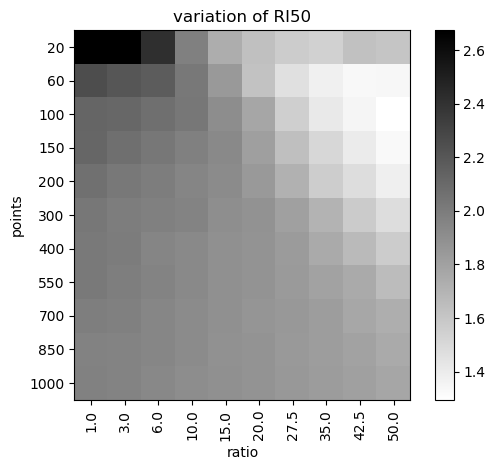
\includegraphics[width = 0.4\linewidth, trim={0 0 0 0}, clip=true]{RI50s_gray.png}
\caption{Dependence of RI50 on number of points added to the grid and ratio of x and y axes for a grid of area $10^6$} (although RI50 is invariant of grid area when using a pointsize of 0).
\label{fig:RI50}
\end{figure}

We observe a large variation in RI50 values with ratio for small n. For ratios near 1, n=20 provides the highest RI50 value which we can rationalize since smaller n leads to more variation between grids and thus a higher 95th percentile value. Surprisingly therefore, we see that n=20 does not correspond to the maximum RI50 for ratios of 15-50.

As we move to higher n, we get less variation between trials and lower RI50 values for the near-square grids.
Higher n-values also exhibit less variability between different ratios with a range of 0.20 for n=1000 compared to 1.13 for n=20 since the proportion of points directly adjacent to an edge decreases with n.

The lowest RI50 values are obtained with relatively small numbers of points (60-100) and high x:y ratios. This is because increasing x:y increases the proportion of points directly adjacent to an edge which increases nearest neighbor variability, particularly for small n.

The reason for the relatively high RI50 values still observed for n=20 is the balance between the increased number of points adjacent to an edge, and the increase in inter-trial variation as we decrease the number of points, This means that even though the median RI50 is lower for n=20 than n=60 for ratios of 20-50, the 95th percentile value is still higher.

\section{Fit to Data}

We load the file spa3\_real.dat and plot the points in figure \ref{fig:ref}. This is the set of reference points (ref) for the remainder of this section

In order to find a set of parameters that generates a distribution of points with similar spatial properties (here represented by RI), we start by defining a spatial similarity measure.

\begin{equation}
u_i = abs(RI(i) - \dfrac{1}{n-1}\sum_{i \neq j}{RI(j)})
\end{equation}

where i=1 specifies the reference grid and i =2:n specifies a set of dmin2d grids generated with a given parameter set.
$u_i$ is thus the difference between the regularity index of grid i and the 99 other grids. We therefore use $u_1$ as a measure of how similar the spatial properties (in this case RI) of the reference grid are to the spatial properties of points positioned with a given set of parameters.
We implement the function \textit{calc\_sim()} which uses this measure to quantify similarity of spatial properties between the reference grid and a set of parameters.

We start by coarsely investigating the parameter space by letting m vary from 0 to 21 and s from 0 to 6.3, quantifying $u_1$ at each point (figure \ref{fig:sim}).

\begin{figure}[h]
	\centering
	\begin{subfigure}[t]{0.38\linewidth}
		\centering
		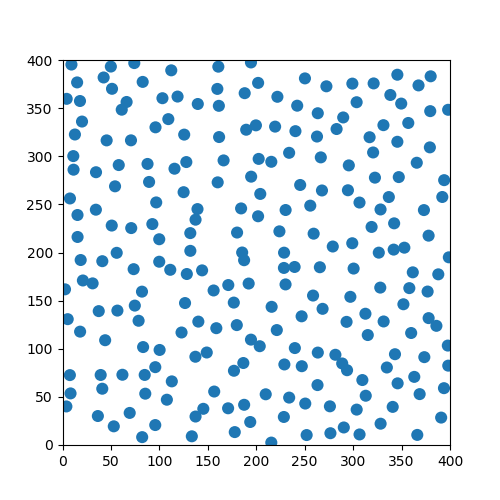
\includegraphics[width = 1.0\linewidth, trim={0 0 0 0}, clip=true]{ref.png}
		\subcaption{set of reference points}
		\label{fig:ref}	
	\end{subfigure}
	\hspace{0.06\linewidth}
	\begin{subfigure}[t]{0.38\linewidth}
		\centering
		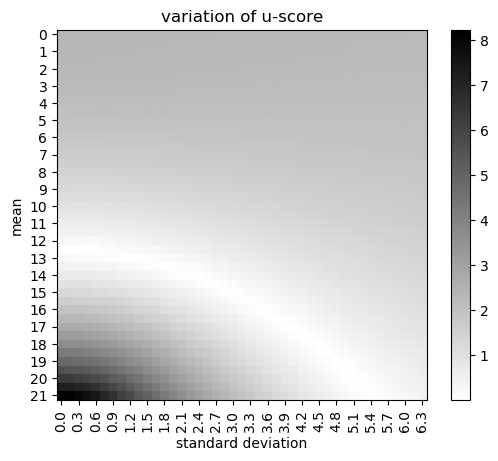
\includegraphics[width = 1.0\linewidth, trim={0 0 0 0}, clip=true]{similarity_gray_good.png}
		\subcaption{$u_1$ for different parameters}
		\label{fig:sim}	
	\end{subfigure}
\label{fig:descent}
\caption{different packings.}
\end{figure}


We see that rather than having a single minimum, there appears to be a line of maximum similarity running from (0.0, 12.5) to (5.5, 21) in a roughly parabolic shape.

Since the $u_1$-landscape appears to be quite well-behaved, we proceed to write a steepest-descent algorithm to find an optimum combination of m and sd to reproduce the spatial properties of the reference grid.

For this minimization, we let the number of grids n used in \textit{calc\_sim()} at each iteration be adaptive rather than fixed at n=100 since we require a higher number of points for an accurate empirical gradient near the minimum.

Since we approach a minimum with $u_1=0$, we let $n = Int(max(5000*exp(-7*u), 20))$ which runs from a minimum value of 20 for $u_1 > 0.55$ to a maximum value of 5000 at $u_1 = 0$.
We also use an adaptive delta ($\delta = u_1/2$) for calculating empirical gradients and an adaptive learning rate ($\epsilon = u_1$).
The standard deviation of $u_1$ across 10 calculations with n=1000 is 0.007 and we thus set a convergence threshold of 0.01 for the optimization.


\begin{figure}[h]
	\centering
	\begin{subfigure}[t]{0.32\linewidth}
		\centering
		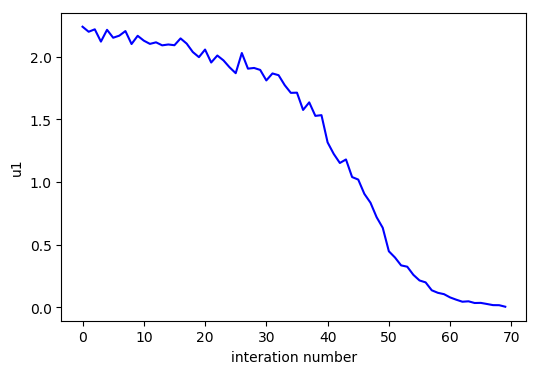
\includegraphics[width = 1.0\linewidth, trim={0 0 0 10}, clip=true]{descent.png}
		\subcaption{$u_1$ as a function of iteration number. The adaptive $\delta$, $\epsilon$ and n result in early steps being rapid and coarse and later steps slower but direct.}
		\label{fig:iter}	
	\end{subfigure}
	\hspace{0.1\linewidth}
	\begin{subfigure}[t]{0.35\linewidth}
		\centering
		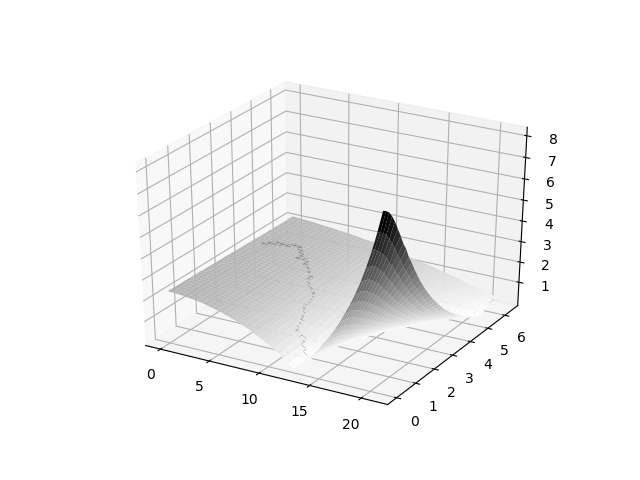
\includegraphics[width = 1.0\linewidth, trim={0 0 0 10}, clip=true]{projected_descent.png}
		\subcaption{projection of steepest descent path onto $u_1$-landscape}
		\label{fig:proj}	
	\end{subfigure}
\label{fig:descent}
\caption{}
\end{figure}

The result of this optimization is m = 12.64 and s = 0.56 giving $u_1 = 0.005$. We see from figure \ref{fig:iter} that the optimization gives a near-monotonic decrease in $u_1$ with each iteration. We take this optimization path and project it onto the $u_1$ landscape from figure \ref{fig:sim} and see that it does indeed proceed in a relatively direct path towards the minimum-u1 valley. Within this valley, it is unlikely that there is a single distinct minimum, and even if there is it is likely not discernable within our error margin.

The steepest descent approach thus allows us to identify a set of parameters yielding similar spatial properties to the real pattern and could be repeated to identify multiple sets of parameters. 
However, since we only have two free parameters and the parameter space is well behaved, in the present case we could identify the line of similarity from an exhaustive search as in figure \ref{fig:sim}.

For a more fine-grained determination of which parameter sets lead to $u_1=0$, we note that each s from 0.0 to 5.5 appears to have a minimum $u_1$ near 0 for an appropriate m. We therefore adapt our steepest descent algorithm to allow for optimization of only the mean given a fixed standard deviation. This allows us to find for each s the m that minimizes $u_1$, and we plot this in figure \ref{fig:msd}.

\begin{figure}[h]
\centering
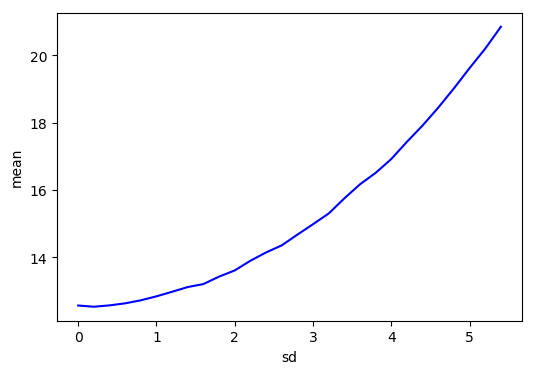
\includegraphics[width = 0.4\linewidth, trim={0 0 0 0}, clip=true]{mean_sd_opt.png}
\caption{optimum mean for different values of s; parameter sets specifying $u_1 = 0$ path}
\label{fig:msd}
\end{figure}

At values of s above 5.5 where the optimum mean goes significantly beyond 20, saturation starts to become a problem and we therefore truncate the curve at 5.4. The curve from s=0.0 to s=5.4 describes a line in parameter space that generates similar spatial properties to those of the reference points.


While we can thus reproduce the regularity index of the reference points with a continuous set of possible parameters, we do note that one could also investigate other constraints to find parameters that produce 'more similar' grids. For example, we see that the optimum m for s=0 is 12.571, but plotting the reference points with a radius of 12.571/2 leads to some degree of overlap, suggesting that these are not the 'real' parameters but that there is some variation in the effective point diameter; i.e. that s is not 0.

Instead, it transpires that the minimum interpoint distance is 8.25 in the reference set of points. We can quantify how many standard deviations 8.25 is from the mean for each parameter set of our optimum-u1 line, and we find that getting dmin=8.25 is most likely for the parameter set (m=16.92, s=4.0) where it is 2.16 standard deviations from the mean. However, further investigations into more complicated similarity measure are beyond the scope of the present report.

\section{Packing density}

We start by considering the theoretical maximum density of points in a 400x400 grid when only the center of a point has to fall in the grid (equivalent to the dmin2d model). An m of 20 in the dmin2d model with zero standard deviation corresponds to packing hard spheres of radius 10. We can imagine two simple systematic ways of doing this; using either a square packing (figure \ref{fig:square}) or a hexagonal packing (figure \ref{fig:hexagonal}), although other 2D bravais lattices also exist.


\begin{figure}[h]
	\centering
	\begin{subfigure}[t]{0.30\linewidth}
		\centering
		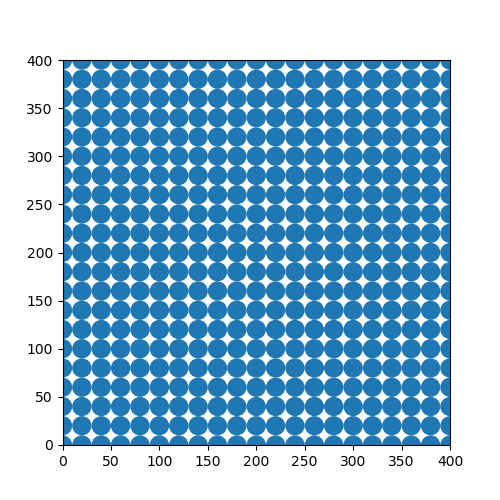
\includegraphics[width = 1.0\linewidth, trim={20 20 20 40}, clip=true]{square.png}
		\subcaption{Square packing of 441 points in a 400x400 grid}
		\label{fig:square}	
	\end{subfigure}
	\hspace{0.16\linewidth}
	\begin{subfigure}[t]{0.30\linewidth}
		\centering
		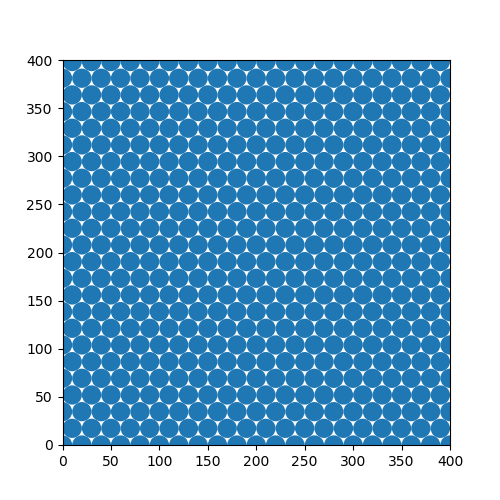
\includegraphics[width = 1.0\linewidth, trim={20 20 20 40}, clip=true]{hexagonal.png}
		\subcaption{Hexagonal packing of 492 points in a 400x400 grid}
		\label{fig:hexagonal}	
	\end{subfigure}
\label{fig:packings}
\caption{}
\end{figure}


In the square packing, we can fit 400/20=20 inter-point distances and thus 21 rows of points in each dimension. This gives a total of 21*21 = 441 points.

With hexagonal packing, the separation between consecutive rows is $\sqrt{20^2-10^2}$. We can thus fit $floor(\dfrac{400}{\sqrt{300}}) = 23$ inter-row distances, corresponding to 24 rows of alternatingly 20 and 21 points in each. This gives a total of
12*(21+20) = 12*41 = 492
points.
We thus find that the theoretical maximum packing density corresponds to 492 points in a 400x400 grid.

In these scenarios, the points extend beyond the 400x400 grid since the dmin2d model only requires the centers of the points to fall within the grid. The real packing density is thus given by the total area of the added points divided by the area of a grid that extends beyond the 400x400 grid by the radius of a point. This gives
$\eta_{sq} = \dfrac{441*10^2*\pi}{420^2} = 78.5\%$ for the square packing and $\eta_{hex}=\dfrac{492*10^2*\pi}{420^2} = 87.6\%$ for the hexagonal packing. Note that these numbers differ from conventional 2D maximum packing densities given the unusual boundary conditions.

To find an empirical measure of 'how many points can be added' with the dmin2d algorithm, we consider an attempt to generate a grid of n points to be failed if 10,000 consecutive points generated do not satisfy the dmin constraint.
We then consider a particular n to be 'over-saturated' or 'unable to add n points' if we fail to generate a grid of n points in 10 consecutive trials.

Given this measure of whether a particular n is 'too high', we write a binary search function \textit{test\_max()} with initial boundary parameters of 0 and 492 to identify $n_{max}$

To asses the reproducibility of this result, we run this binary search algorithm 10 times with the function \textit{repeat\_max()} and arrive at the following $n_{max}$ values:
[290,
294,
292,
290,
287,
294,
292,
289,
292,
294].\\
A reasonable estimate of when we cannot add more points in a dmin2d() framework is thus 294 points.

We also implement the 'birth and death' model specified in the assignment in the function \textit{birth\_death\_model()}. We modify \textit{test\_max()} above to run 10 binary seaches of 'birth and death saturation', considering an attempt to generate a grid failed if we fail to add a point 10,000 consecutive times in any epoch, and an n to be saturated if we fail to generate a grid 10 consecutive times.
This gives  $n_{max}$ of
[300,
301,
304,
297,
302,
302,
300,
298,
302,
298].\\
We therefore take 302 as the maximum number of points that can be added using the birth and death model. We thus see that the birth and death model consistently packs more points than the sequential model by generating more regularly spaced points for a given n.

\begin{figure}[h]
	\centering
	\begin{subfigure}[t]{0.30\linewidth}
		\centering
		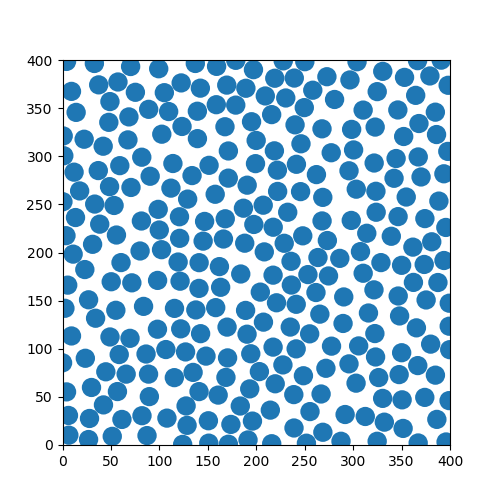
\includegraphics[width = 1.0\linewidth, trim={20 20 20 40}, clip=true]{plot_seq294.png}
		\subcaption{294 points generated by the sequential algorithm}
		\label{fig:dminmax}	
	\end{subfigure}
	\hspace{0.16\linewidth}
	\begin{subfigure}[t]{0.30\linewidth}
		\centering
		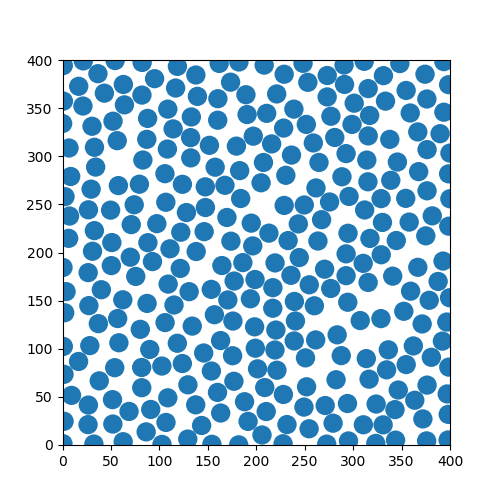
\includegraphics[width = 1.0\linewidth, trim={20 20 20 40}, clip=true]{plot_bd302.png}
		\subcaption{302 points generated by the epoch algorithm}
		\label{fig:bdmax}	
	\end{subfigure}
\label{fig:models}
\caption{}
\end{figure}


We plot an example of a 294-point grid generated by the dmin2d model and a 302-point grid generated by the birth and death model in figures  \ref{fig:dminmax} and \ref{fig:bdmax}.
There appear to be small areas where an additional point could be added, suggesting that the calculated values are not hard ceilings; but they do provide an empirical estimate of what's feasible within a reasonable timeframe. The corresponding packing densities are $\eta_{dmin2d} = 52.3\%$ and $\eta_{bd} = 53.8\%$.

We also note that both the 294 points added by the dmin2d model and the 302 points added by the epoch model are very much lower than the theoretical maximum packing of 492 points. This suggests that these are not good models for simulating dense-packing systems such as crystals.
However, they may be more applicable for biological systems with smaller 'penalties' for non-regularity.




\section{Moving points}

We implement the Lubachevsky-Stillinger (LS) model in the function \textit{LS\_model()}  as described in their 1990 paper, at every timepoint predicting the next event that will take place and updating the system accordingly. We terminate the simulation when we reach a maximum number of iterations or when the next predicted event leads to disk overlap (this can occur in jammed states given numerical inaccuracies). We also re-normalize all velocites once the mean speed of the particles exceeds 10 (this value was determined empirically). Initial velocities have components generated uniformly at random between -1 and 1, and the size of all disks grows at a constant rate such that their diameter a is given by $a(t) = a_0t$ as described by Lubachevsky and Stillinger.

For comparison with the above results, we use a 420x420 grid for all Lubachevsky-Stillinger simulations since that is the effective space taken up by the r=10 disks in the dmin2d-generated 400x400 grid. As noted in the discussion above, it is not possible in the dmin2d model to have the center of a sphere beyond the 400x400 grid, making the present scenario slightly different. However, given the inherent differences in boundary conditions, we consider this the best approximation to a fair comparison. The overall conclusions will be invariant to small differences in the definition of packing densities.

We start by verifying the algorithm with a0=2.5 for n=12 (figure \ref{fig:12}) and n=24 (figure \ref{fig:24}) points. For n=12, this leads to a slightly elongated hexagonal packing with a final disk radius of 62.92, giving a packing density of 84.6\% which is similar to the hexagonal packing density above.

For n=24, we similarly observe a rotated and slightly elongated hexagonal packing with a final disk radius of 44.59 giving a packing density of 85.0\%. These values are not quite as high as the hexagonal packing density above, a consequence of the fact that we cannot achieve perfect hexagonal packing in a square grid, and the smaller disk size in figure \ref{fig:hexagonal} reduces the error. We note that both of the packing densities reported here are much higher than was the case for the patterns generated using dmin2d and the birth and death model, and begin to approach the upper packing density limits. When running LS simulations for small n not of the form $n=n_1*n_2$ with $n_1 \approx n_2$, packings are generally less regular with lower packing densities as also described by Lubachevsky and Stillinger.

\begin{figure}[h]
	\centering
	\begin{subfigure}[t]{0.30\linewidth}
		\centering
		%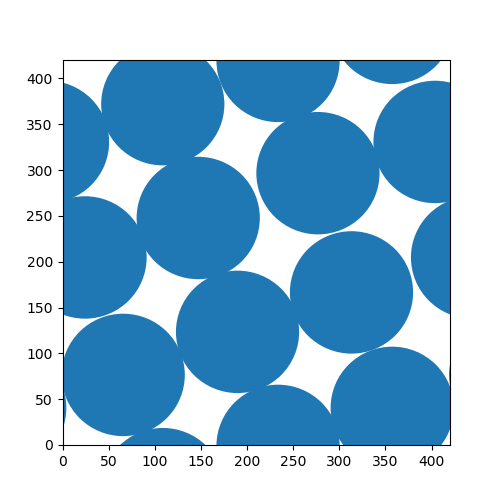
\includegraphics[width = 1.0\linewidth, trim={20 20 20 20}, clip=true]{temp/jammed_10.png}
		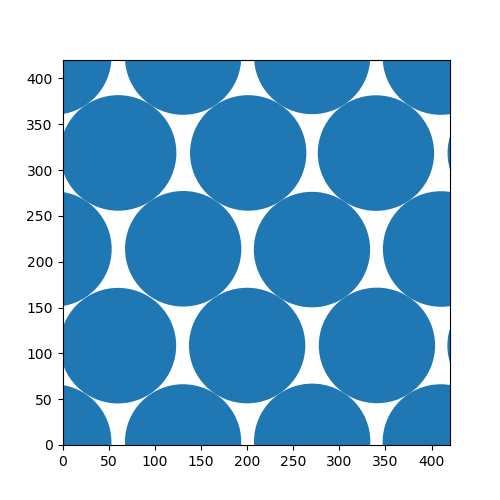
\includegraphics[width = 1.0\linewidth, trim={20 20 20 20}, clip=true]{temp/jammed_12_12584.png}
		\subcaption{n=12, a0=2.5, r=62.92 }
		\label{fig:12}	
	\end{subfigure}
	\hspace{0.0005\linewidth}
	\begin{subfigure}[t]{0.30\linewidth}
		\centering
		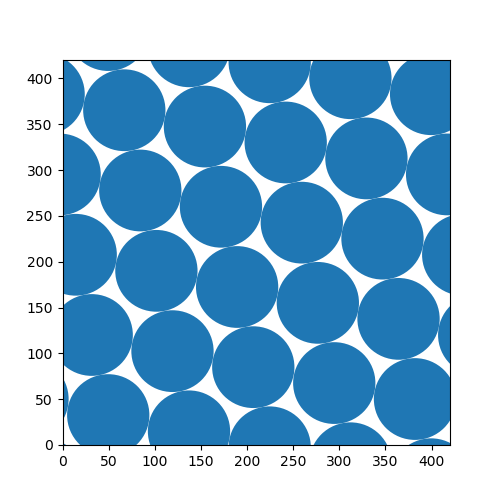
\includegraphics[width = 1.0\linewidth, trim={20 20 20 20}, clip=true]{temp/24_pack_end.png}
		\subcaption{n=24, a0=2.5, r=44.59}
		\label{fig:24}	
	\end{subfigure}
	\hspace{0.0005\linewidth}
	\begin{subfigure}[t]{0.30\linewidth}
		\centering
		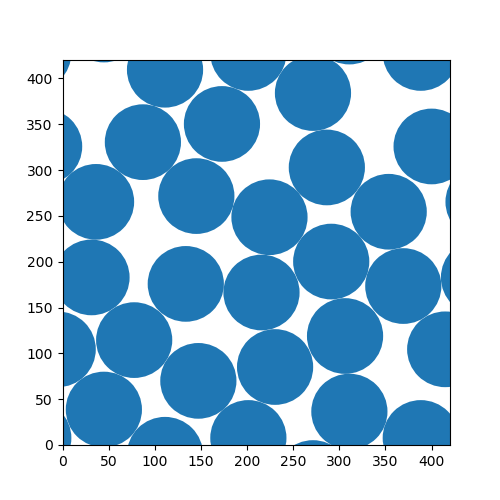
\includegraphics[width = 1.0\linewidth, trim={20 20 20 20}, clip=true]{temp/24_irregular.png}
		\subcaption{n=24, a0=4.5, r=44.59}
		\label{fig:24high}	
	\end{subfigure}
\label{fig:models}
\caption{End-results of Lubachevsky-Stillinger simulations for different numbers of points and growth rates. Note that the grids have been plotted with periodic boundary conditions in contrast to previous plots in the report.}
\end{figure}

Similar to the observations of Lubachevsky and Stillinger, we observe that upon increasing the growth rate from 2.5 to 4.5, irregular jammed final states become more prevalent than regular packings (figure \ref{fig:24high}).
For n=24 and a0=4.5, we thus observe a final disk radius of 41.29 giving a packing density of 72.9\%, which is much lower than that obtained with a smaller growth rate.

To further verify that the implementation works as expected, we can investigate in more detail the path to jammed packing in figure \ref{fig:24}. We thus plot the state of the simulation at four different timespoints in figures \ref{fig:24_1}-\ref{fig:24_4}.
We see that the points start out by being scattered at random, but as they grow and collide they form a more lattice-like structure. In figure \ref{fig:24_3}, we see the beginnings of the pseudo-hexagonal lattice that has fully formed by the end of the simulation.

\begin{figure}[h]
	\centering
	\begin{subfigure}[t]{0.24\linewidth}
		\centering
		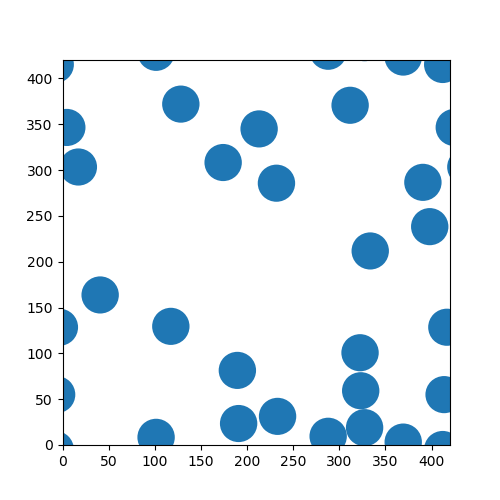
\includegraphics[width = 1.0\linewidth, trim={20 20 20 20}, clip=true]{temp/24_pack_4051.png}
		\subcaption{pointsize 20.25}
		\label{fig:24_1}	
	\end{subfigure}
	\hspace{0.0005\linewidth}
	\begin{subfigure}[t]{0.24\linewidth}
		\centering
		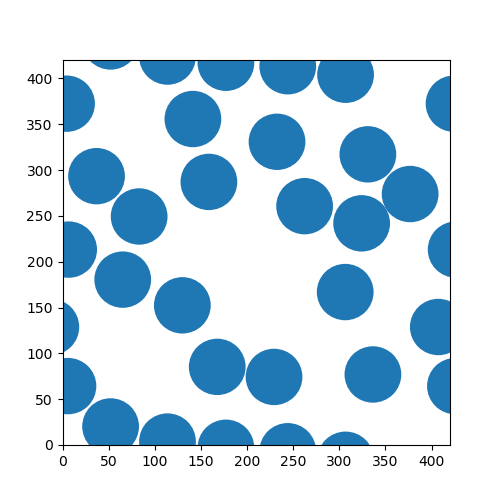
\includegraphics[width = 1.0\linewidth, trim={20 20 20 20}, clip=true]{temp/24_pack_6152.png}
		\subcaption{pointsize 30.76}
		\label{fig:24_2}	
	\end{subfigure}
	\hspace{0.0005\linewidth}
	\begin{subfigure}[t]{0.24\linewidth}
		\centering
		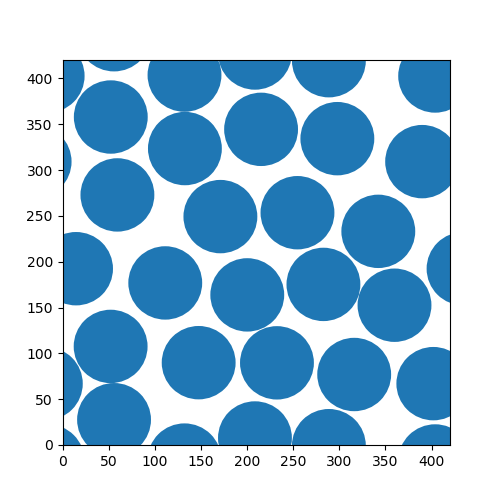
\includegraphics[width = 1.0\linewidth, trim={20 20 20 20}, clip=true]{temp/24_pack_8006.png}
		\subcaption{pointsize 40.03}
		\label{fig:24_3}	
	\end{subfigure}
	\hspace{0.0005\linewidth}
	\begin{subfigure}[t]{0.24\linewidth}
		\centering
		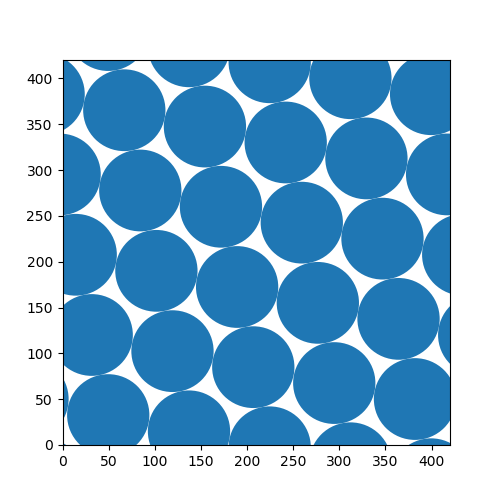
\includegraphics[width = 1.0\linewidth, trim={20 20 20 20}, clip=true]{temp/24_pack_end.png}
		\subcaption{pointsize 44.59}
		\label{fig:24_4}	
	\end{subfigure}
\label{fig:models}
\caption{Freeze frames of a single Lubachevsky-Stillinger simulation with n=24 on a square lattice.}
\end{figure}

To quantify the number of radius 10 points we can fit on a grid with the LS-model compared to the dmin2d and birth and death models above, we add points to a 420x420 grid and terminate a simulation of n disks when they reach a diameter of 20 since this is equivalent to having added n points with dmin=20 to the grid. 

We consider an attempt to be failed if the size of the points asymptotes before reaching 20. We use $a_0 = 1.0$ as this should lead to regular packings according to Lubachevsky \& Stillinger and the simulations above.

A binary search approach similar to the one described in section 4 leads to  $n_{max} = 408$, and three frames of this simulation have been plotted in figures \ref{fig:sat_1}-\ref{fig:sat_3}.

\begin{figure}[h]
	\centering
	\begin{subfigure}[t]{0.31\linewidth}
		\centering
		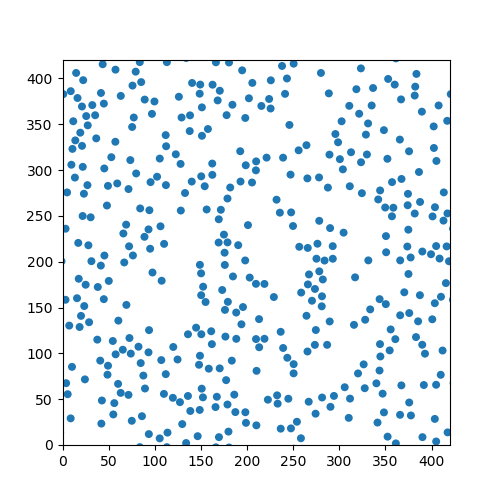
\includegraphics[width = 1.0\linewidth, trim={20 20 20 20}, clip=true]{temp/408_opt_865.png}
		\subcaption{pointsize 4.3}
		\label{fig:sat_1}	
	\end{subfigure}
	\hspace{0.01\linewidth}
	\begin{subfigure}[t]{0.31\linewidth}
		\centering
		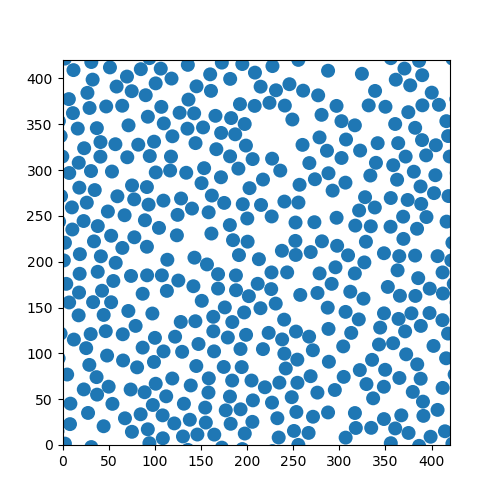
\includegraphics[width = 1.0\linewidth, trim={20 20 20 20}, clip=true]{temp/408_opt_1518.png}
		\subcaption{pointsize 7.6}
		\label{fig:sat_2}	
	\end{subfigure}
	\hspace{0.02\linewidth}
	\begin{subfigure}[t]{0.31\linewidth}
		\centering
		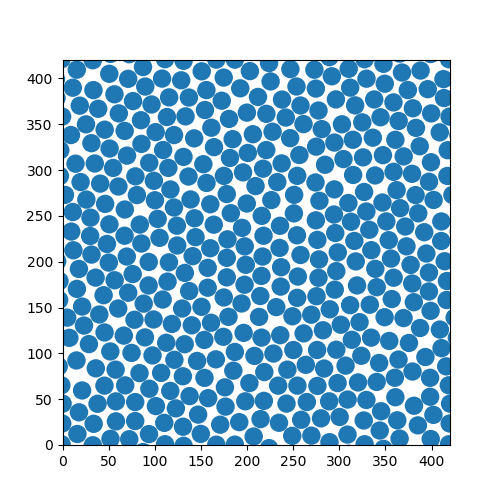
\includegraphics[width = 1.0\linewidth, trim={20 20 20 20}, clip=true]{temp/408_opt_200.png}
		\subcaption{pointsize 10.0}
		\label{fig:sat_3}	
	\end{subfigure}
\label{fig:models}
\caption{different packings.}
\end{figure}

We note that for $n_{max}$, most of the points do not appear to be completely jammed in contrast to our observations for n=12 and n=24. This could be a result of the parameters needing further tweaking for higher n or due to numerical instabilities in the present implementation. We would imagine that if we ran the algorithm for long enough with suitable parameters (i.e. infinitesimal a0 for infinite time), we would again achieve a hexagonal packing with a packing density close to the theoretical maximum of $\dfrac{\pi}{2*\sqrt{3}} = 90.7\%$ (although this is a limit as n goes to infinity for a square lattice).

The combination of growth and repulsion observed in the Lubachevsky-Stillinger Model may be more useful for modelling a range of biological systems than the dmin2d model with spontaneuous appearance of elements. For example, growth of neurons is known to involve continuous growth combined with seceretion of inhibitory factors preventing excessive parallel growth of neurons.

Similarly, neuroblast development in \textit{Drosophila} involves notch-delta-mediated lateral inhibition between nascent neuroblasts and neighboring cells, leading to a series of regularly spaced neuroblasts for subsequent generation of Ganglion Mother Cells. This could potentially also be modelled in a slightly  modified Lubachevsky-Stillinger framework with the increasing disk size representing the extent of inhibition.

On an organism-wide level, we could also imagine using the Lubachevsky-Stillinger model to model growth of single celled organisms such as bacteria or yeast, with nodes representing individual colonies. In this case, we could allow for more complex interactions between points and different pointsizes.

One disadvantage of the LS model for biological systems is that it requires a fixed n which is often not the case in real systems, where the appearance or lack of appearance of an additional 'point' (e.g. cell, colony or organism) might depend on the degree of inhibition and effective size of other points. A lot of biological systems thus involve a combination of interactions between nodes, growth of nodes, and sequential addition of nodes. None of the three models considered in the present report captures all of these properties.


\section{Appendix (code)}

\lstset{basicstyle=\footnotesize}

\large{File: sp3.jl}
\lstinputlisting[language=python]{sp3.jl}

\large{File: dmin2d.jl}
\lstinputlisting[language=python]{dmin2d.jl}

\large{File: RI50.jl}
\lstinputlisting[language=python]{RI50.jl}

\large{File: saturation.jl}
\lstinputlisting[language=python]{saturation.jl}

\large{File: birth\_death.jl}
\lstinputlisting[language=python]{birth_death.jl}

\large{File: LS\_model.jl}
\lstinputlisting[language=python]{LS_model.jl}

\end{document}

